\documentclass[border=4pt]{standalone}
\usepackage{amsmath,amssymb,pgfplots}\pgfplotsset{compat=1.18}
\definecolor{figB}{RGB}{31,90,166}\definecolor{figR}{RGB}{176,48,48}\definecolor{figG}{RGB}{46,125,50}\definecolor{figO}{RGB}{214,120,20}
% dim null T^k = 0,3,5,6,6,...; the red part of bar k is the jump dim null T^k - dim null T^{k-1}.
\begin{document}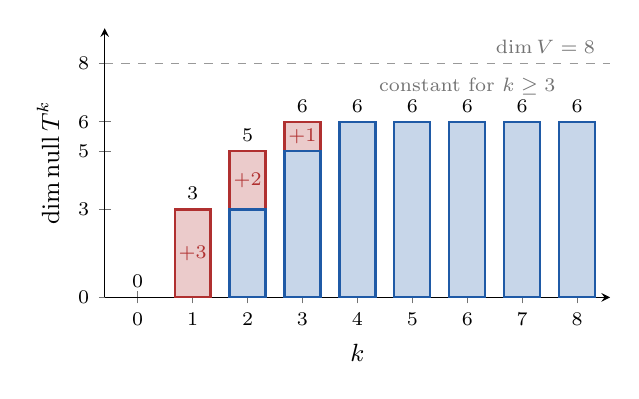
\begin{tikzpicture}
\begin{axis}[width=8cm,height=5cm,ybar stacked,bar width=13pt,ymin=0,ymax=9.2,xmin=-0.6,xmax=8.6,
 axis lines=left, axis line style={-stealth,thin}, tick style={thin,black!55}, ticklabel style={font=\scriptsize},
 xtick={0,...,8},ytick={0,3,5,6,8},xlabel={$k$},ylabel={$\dim\operatorname{null}T^k$},label style={font=\small}]
\addplot[fill=figB!25,draw=figB,thick] coordinates {(0,0)(1,0)(2,3)(3,5)(4,6)(5,6)(6,6)(7,6)(8,6)};
\addplot[fill=figR!25,draw=figR,thick] coordinates {(0,0)(1,3)(2,2)(3,1)(4,0)(5,0)(6,0)(7,0)(8,0)};
\draw[dashed,black!40,thin] (axis cs:-0.6,8)--(axis cs:8.6,8);
\node[font=\scriptsize,black!55,anchor=south east] at (axis cs:8.5,8) {$\dim V=8$};
\coordinate (j1) at (axis cs:1,1.5);
\coordinate (j2) at (axis cs:2,4);
\coordinate (j3) at (axis cs:3,5.5);
\node[font=\scriptsize,anchor=south] at (axis cs:1,3) {$3$};
\node[font=\scriptsize,anchor=south] at (axis cs:2,5) {$5$};
\node[font=\scriptsize,anchor=south] at (axis cs:3,6) {$6$};
\node[font=\scriptsize,anchor=south] at (axis cs:4,6) {$6$};
\node[font=\scriptsize,anchor=south] at (axis cs:5,6) {$6$};
\node[font=\scriptsize,anchor=south] at (axis cs:6,6) {$6$};
\node[font=\scriptsize,anchor=south] at (axis cs:7,6) {$6$};
\node[font=\scriptsize,anchor=south] at (axis cs:8,6) {$6$};
\node[font=\scriptsize,anchor=south] at (axis cs:0,0) {$0$};
\node[font=\scriptsize,black!55] at (axis cs:6,7.2) {constant for $k\ge3$};
\end{axis}
\foreach \j/\t in {1/3,2/2,3/1} \node[font=\scriptsize,figR] at (j\j) {$+\t$};\end{tikzpicture}\end{document}
